Die  \emph{View} ist  aus  zwei \"ubergeordneten  Panels aufgebaut. Im  linken
Panel  befinden  sich  Ein-  und Ausgabefelder  f\"ur  numerische  Werte,  das
rechte  Panel  beheimtated  die  Plots  sowie  das  Optimierungs-Panel  (siehe
Abbildung~\ref{fig:toolStartPI}).

\begin{figure}[h!, width=\pagewidth]
    \centering
    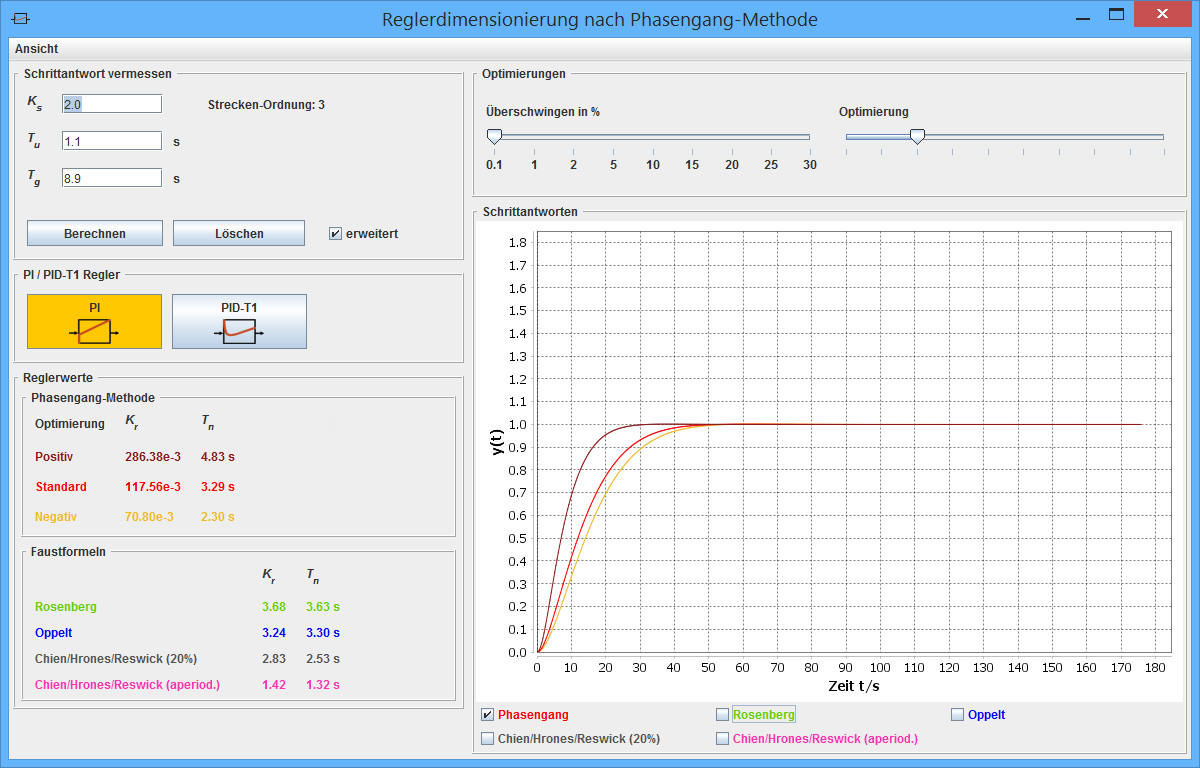
\includegraphics[width=0.9\textwidth]{images/toolStartPI.jpg}
    \caption{Grundlegender Aufbau der Benutzeroberfl\"ache}
    \label{fig:toolStartPI}
\end{figure}

Das    rechte   Panel    kann   mittels    der   Check-Box    \emph{erweitert}
(Abbildung~\ref{fig:toolStartPIDSmallErweitert})    ein-   und    ausgeblendet
werden,       die      reduzierte       Benutzeroberfl\"ache      ist       in
Abbildung~\ref{fig:toolStartPIDSmall} zu sehen.

\begin{minipage}[t][][b]{0.45\textwidth}
    \centering

    \begin{minipage}[c][][b]{\textwidth}
        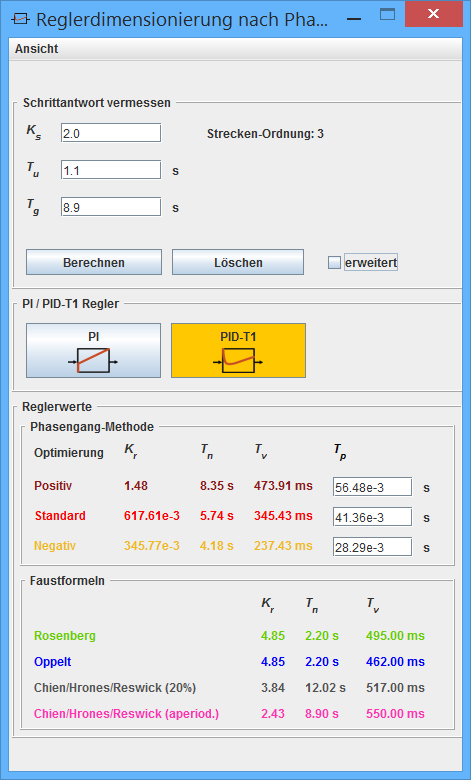
\includegraphics[width=\textwidth]{images/toolStartPIDSmall.jpg}
        \captionof{figure}{Benutzeroberfl\"ache reduziert auf linkes Panel}
        \label{fig:toolStartPIDSmall}
    \end{minipage}

    \begin{minipage}[c][][b]{\textwidth}
        \centering
        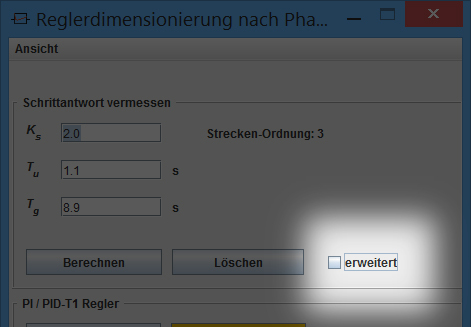
\includegraphics[width=\textwidth]{images/toolStartPIDSmallErweitert.jpg}
        \captionof{figure}{Checkbox zum Zu- und Wegschalten des rechten Haupt-Panels}
        \label{fig:toolStartPIDSmallErweitert}
    \end{minipage}

\end{minipage}
\begin{minipage}[t][][b]{0.45\textwidth}
    \centering
    \begin{minipage}[c][][b]{\textwidth}
        \centering
        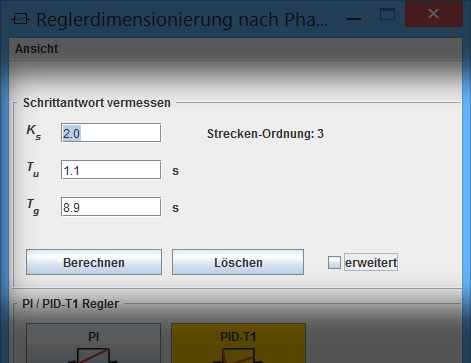
\includegraphics[width=\textwidth]{images/toolStartPIDSmallSchrittantwort.jpg}
        \captionof{figure}{Bereich zum Eingeben der Streckenparameter}
        \label{fig:toolStartPIDSmallSchrittantwort}
    \end{minipage}

    \begin{minipage}[c][][b]{\textwidth}
        \centering
        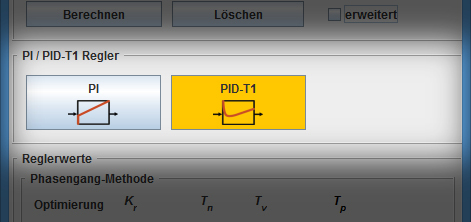
\includegraphics[width=\textwidth]{images/toolStartPIDSmallButtons.jpg}
        \captionof{figure}{Auswahl zwischen PI- und PID-Regler}
        \label{fig:toolStartPIDSmallButtons}
    \end{minipage}

    \begin{minipage}[c][][b]{\textwidth}
        \centering
        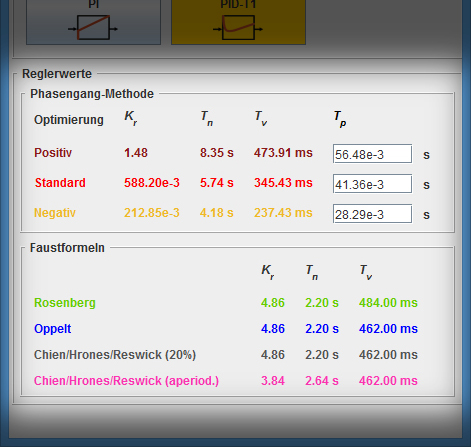
\includegraphics[width=\textwidth]{images/toolStartPIDSmallRegler.jpg}
        \captionof{figure}{Ausgabewerte des dimensionierten Reglers}
        \label{fig:toolStartPIDSmallRegler}
    \end{minipage}

\end{minipage}

Im             Bereich             \emph{Schrittantwort             vermessen}
(Abbildung~\ref{fig:toolStartPIDSmallSchrittantwort}) werden die Parameter der
vermessenen  Strecke eingegeben. Darunter  befinden sich  die Schalftfl\"achen
zur   Wahl   zwischen  der   Dimensionierung   eines   PI-  respektive   eines
PID-T1-Reglers (Abbildung~\ref{fig:toolStartPIDSmallButtons}).

Das  Panel   \emph{Reglerwerte}  (Abbildung~\ref{fig:toolStartPIDSmallRegler})
dient   der   Ausgabe   der    berechneten   Reglerwerte   der   verschiedenen
Berechnungsmethoden. Ebenfalls  kann f\"ur  die Phasengangmethode,  sofern ein
PID-Regler dimensioniert wird, die  Zeitkonstante $T_p$ spezifiziert werden.

Das  Optimierungs-Panel  (Abbildung~\ref{fig:optimierungen}  )beinhaltet  zwei
Slider  zur  Eingabe  des   gew\"unschten  \"Uberschwingens  respektive  f\"ur
die  Optimierung   des  Reglers  der  Phasengangmethode. \"Uber   den  Slider
\emph{Optimierung} kann $\varphi_r$ beeinflusst werden.

\begin{figure}[h!, width=\pagewidth]
    \centering
    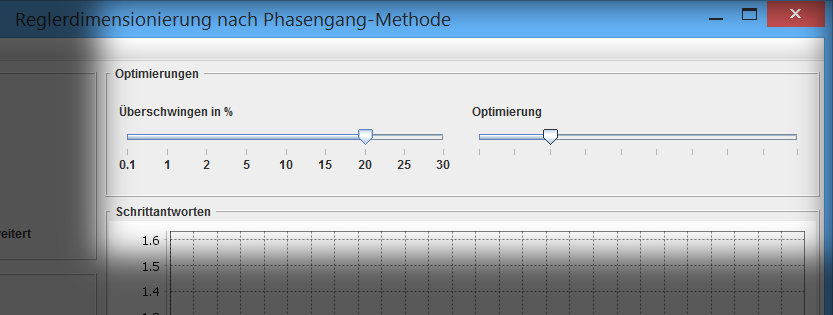
\includegraphics[width=0.6\textwidth]{images/tool20UeberschwingenPIDOptimierungen.jpg}
    \caption{Slider im Optimierungs-Panel}
    \label{fig:optimierungen}
\end{figure}

\begin{figure}[h!, width=\pagewidth]
    \centering
    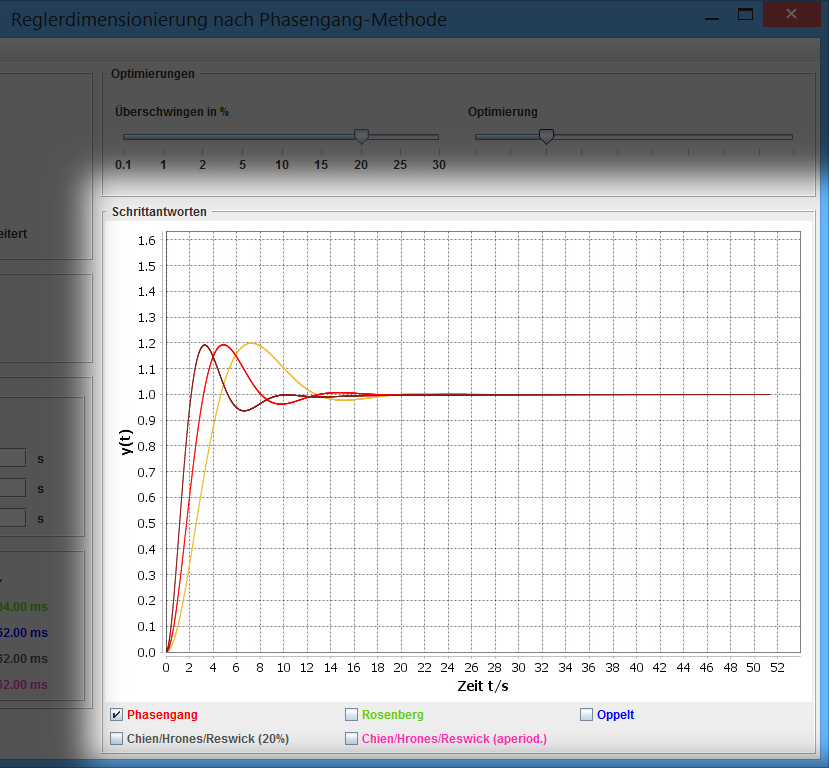
\includegraphics[width=0.6\textwidth]{images/tool20UeberschwingenPIDPlots.jpg}
    \caption{Plots der Schrittantworten, PID-Regler berechnet nach Phasengangmethode, 20\% \"Uberschwingen}
    \label{fig:tool20Plots}
\end{figure}

Unterhalb des  Optimierungs-Panels werden  die Plots der  mittels Faustformeln
und  Phasengangmethode   errechneten  Schrittantworten   graphisch  ausgegeben
(Abbildung~\ref{fig:tool20Plots}). Diese  k\"onnen   mittels  Check-Boxen  zu-
und   weggeschaltet  werden   (Bereich  entlang   des  unteren   Bildrands  in
Abbildung~\ref{fig:tool20Plots}).

Die Resultate der Phasengangmethode werden durch drei Kurven dargestellt. Eine
Kurve   benutzt  den   Standardwert  f\"ur   $\varphi_r$  gem\"ass   Zellweger
($-90\degree$  f\"ur PI-Regler,  $-135\degree$ f\"ur  PID-Regler), die  beiden
anderen Kurven  basieren auf Benutzereingaben  f\"ur einen oberen  und unteren
Offset  von  $\varphi_r$,  der   \"uber  den  Schiebregler  \emph{Optimierung}
eingestellt       werden       kann. Das       Ergebnis       kann       unter
anderem      in     Abbildung~\ref{fig:comparisonPID002optimisations}      auf
Seite~\pageref{fig:comparisonPI015} gesehen werden.

Es   ist   ebenfalls   m\"oglich,   die   dargestellten   Plots   als   Bilder
zu   speichern;   die    in   Abschnitt~\ref{subs:tool:results}   abgebildeten
Beispiele   (Abbildungen~\ref{fig:comparisonPI015},~\ref{fig:comparisonPID015}
und~\ref{fig:comparisonPID002optimisations} auf Seite~\pageref{fig:comparisonPI015})
wurden mit unserem Tool erstellt und exportiert.

\clearpage
